%%%%%%%%%%%%%%%%%%%%%%%%%%%%%%%%%%%%%%%%%%%%%%%%%%%%%%%%%%%%%%%%%%%
%                                                                 %
%                            CHAPTER SIX                          %
%                                                                 %
%%%%%%%%%%%%%%%%%%%%%%%%%%%%%%%%%%%%%%%%%%%%%%%%%%%%%%%%%%%%%%%%%%%

\chapter{ONTOLOGY VERSIONING}

\section{Sea Ice Ontology}

A great many annotations were made to Version 2 of the Sea Ice Ontology.
Maintaining those notes after migration to the new version would provide great value to the project.
From the color code in Table \ref{ColorTable}, yellow and blue changes correspond directly to Modification and Addition transitions, respectively.
In theory, the green concepts would also qualify for a Modify categorization since they would likely have a new URI, meaning that an attribute exists between two versions and something has changed.
However, this would result in a product that is at least the size of the union of the two versions, greatly hindering the scalability of the approach.
The obvious solution would be to leave the attributes unlinked, as in the approach with the spreadsheet application where no change was detected.
The Invalidation change would cover concepts which do not have a mapping into Version 3.
Therefore, the remaining transition types, purple and red require more specific attention than a usual Modify.

\begin{table}
	\newcommand*{\thead}[1]{\multicolumn{1}{|c|}{\bfseries #1}}
	\centering
	\begin{tabular}{ | c | l |}
		\hline
		\textbf{Color} & \thead{Description} \\
		\hline
		Purple & Moved since the previous version of the ontology.\\
		\hline
		Green & Still the same.\\
		\hline
		Yellow & In the same place; but perhaps the name or definition have changed.\\
		\hline
		Red & Suggest changes to be made to both the ontologies and the nomenclature.\\
		\hline
		Blue & New concepts to be added to the ontologies.\\
		\hline
	\end{tabular}
	\label{ColorTable}
	\caption{Color code used by the concept maps made by Ruth Duerr during the planning phase of the Sea Ice Ontology's development.}
\end{table}

\section{GCMD Keywords}

\subsection{Creating the Versioning Graph}

The keywords can be acquired in a number of different formats, but the one chosen was RDF.  In the file, each concept uses a unique URI as an identifier and uses the concepts skos:Broader and skos:Narrower to establish the hierarchy.  When the GCMD group release a new version, they reuse the same URI for reused concepts.  To create a mapping, new and old concepts can be easily filtered out by finding URIs which are also skos:Concepts but only exist in one version or the other.  The remaining concepts must therefore be modification changes or unchanged.  Since, the primary data the hierarchy contains is its parent and children nodes, modifications occur when the concept moves around in the hierarchy.  To determine this, the values of a concept's skos:Broader relationship is checked.

Since the URIs are reused, the history of a concept can be tracked through the versioned lifespan of the concept.

\begin{figure}%[b]
	\centering
	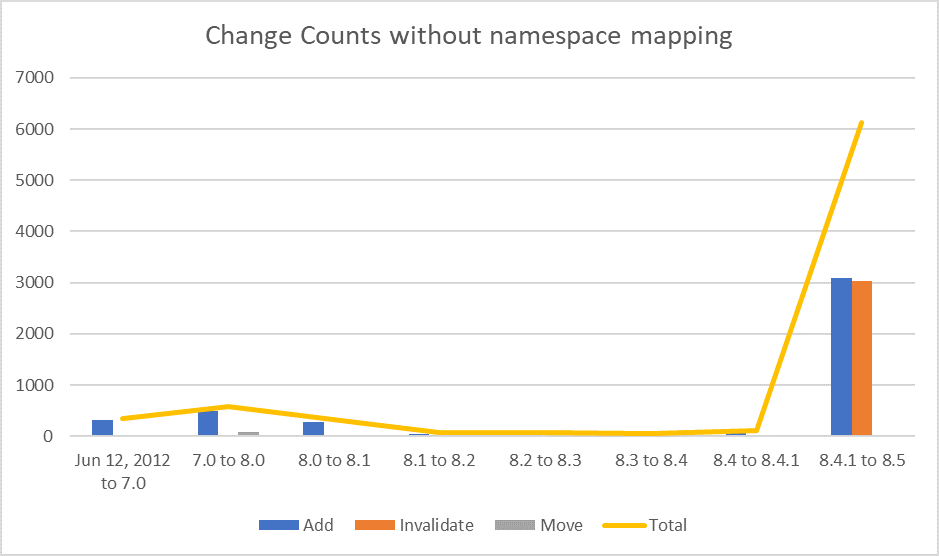
\includegraphics[scale=1]{figures/GCMDChart1.png}
	\caption{Add, Invalidate, and Modify counts in Version 8.5.  The counts show change magnitudes and indicate that major and minor changes differ by orders of magnitude.}
	\label{GCMDC1}
\end{figure}

In Figure \ref{GCMDC1}, we can see that changing from version 8.4.1 to 8.5, there is a large spike in changes.  Note that the number of each adds and invalidates number to approximately the size of the entire keyword list.  This is a result of a NASA policy change requiring web resources to use the https protocol.  As a result, all the URIs of the concepts changed, and the entire list was essentially removed and then re-added.  Without the breakdown of the magnitude of changes into the three subtypes, the total reported change would be both difficult to interpret and exceed the size of the dataset significantly.

In Figure \ref{GCMDC2}, we can see an accounting of the changes with the URI namespace.  After controlling for the namespace change, we can see that the dataset is dominated by add changes.  In addition, in migrations across major numbers, the magnitude of adds range in the hundreds.  This is an order of magnitude different than the numbers of add changes while stepping across minor number differences.  From the identifier scheme and the change counts, it is clear that the keyword management team expected only minor changes and names the version as such even though changes to namespace constitute significant differences according to linked data definitions.

\begin{figure}%[b]
	\centering
	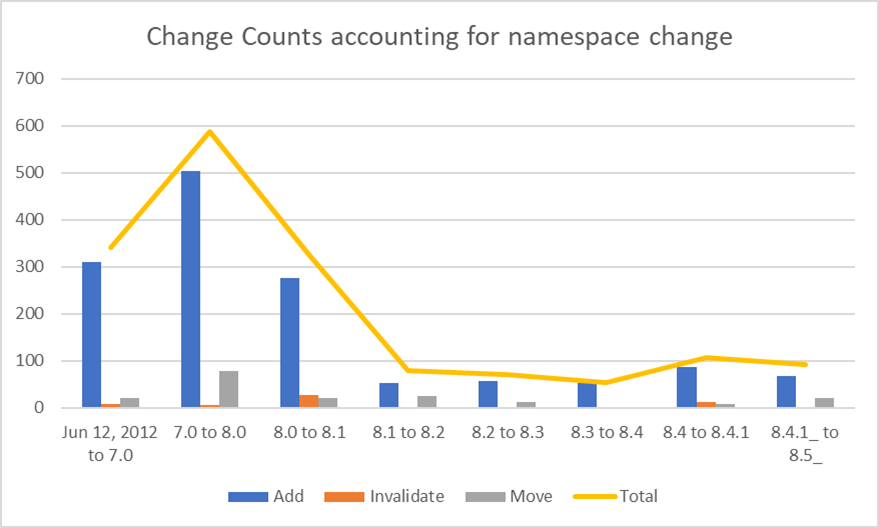
\includegraphics[scale=1]{figures/GCMDChart2.png}
	\caption{Add, Invalidate, and Modify counts ignoring the namespace changes in Version 8.5.  The counts show change magnitudes appropriate for the identifier.}
	\label{GCMDC2}
\end{figure}